\documentclass{article}
\usepackage{listings}
\usepackage{mathrsfs}
\usepackage[utf8]{inputenc}
\usepackage{amssymb}
\usepackage{lipsum}
\usepackage{amsmath}
\usepackage{fancyhdr}
\usepackage{geometry}
\usepackage{scrextend}
\usepackage[english,german]{babel}
\usepackage{titling}
\setlength{\droptitle}{-3cm}
\usepackage{tikz}
\usepackage{algorithm,algpseudocode}
\usepackage[doublespacing]{setspace}
\usetikzlibrary{datavisualization}
\usetikzlibrary{datavisualization.formats.functions}
\usepackage{polynom}
\usepackage{amsmath}
\usepackage{gauss}
\usepackage{tkz-euclide}
\usetikzlibrary{datavisualization}
\usetikzlibrary{datavisualization.formats.functions}
\author{
Alexander Mattick Kennung: qi69dube\\
Kapitel 1
}
\usepackage{import}
\date{\today}
\geometry{a4paper, margin=2cm}
\usepackage{stackengine}
\parskip 1em
\newcommand\stackequal[2]{%
  \mathrel{\stackunder[2pt]{\stackon[4pt]{=}{$\scriptscriptstyle#1$}}{%
  $\scriptscriptstyle#2$}}
 }
\makeatletter
\renewcommand*\env@matrix[1][*\c@MaxMatrixCols c]{%
  \hskip -\arraycolsep
  \let\@ifnextchar\new@ifnextchar
  \array{#1}}
\makeatother
\lstset{
  language=haskell,
}
\lstnewenvironment{code}{\lstset{language=Haskell,basicstyle=\small}}{}
\usepackage{enumitem}
\setlist{nosep}
\usepackage{titlesec}

\titlespacing*{\subsection}{0pt}{2pt}{3pt}
\titlespacing*{\section}{0pt}{0pt}{5pt}
\titlespacing*{\subsubsection}{0pt}{1pt}{2pt}
\title{Vorlesung 4}


\begin{document}
	\maketitle
	zuerst die Beta(3,1)-Verteilung:\\
	\[f_1(x)=\frac{1}{B(3,1)}x^{3-1}(1-x)^{1-1}\]
	\[B(3,1)=\frac{\Gamma(1)\Gamma(3)}{\Gamma(3+1)}\]
	Ganze zahlen, also auf Fakultät reduzierbar:\\
	\[B(3,1)=\frac{(1-1)!(3-1)!}{3!}\]
	\[B(3,1)=\frac{1*2}{6}\]
	\[B(3,1)=\frac{1}{3}\]
	Daraus folgt die wahrscheinlichkeitsdichtefunktion:\\
	\[f_1(x_1)=\begin{cases}3x_1^2&x_1\in[0,1]\\0&sonst\end{cases}\]
	Der Rand kann mit eingeschlossen werden, da $3\geq 1\land 1\geq 1$ ist.\\
	Die Gleichverteilung ist so definiert, dass\\
	\[p(x)=p(y), \forall x,y\in[0,\frac{x_1}{2}]\]
	ist.\\
	als Formel also:
	\[f^1_2(x_2;x_1) = \begin{cases}\frac{1}{\frac{f_1(x_1)}{2}}&x_2\in[0,\frac{f_1(x_1)}{2}]\\0&sonst\end{cases}\]
	\[f^1_2(x_2;x_1) = \begin{cases}\frac{2}{3x_1^2}&x_2\in[0,\frac{3x_1^2}{2}]\\0&sonst\end{cases}\]
	Der gesamtversuch besteht aus beiden Teilvesuchen:
	\[f(x_1,x_2) = f_1(x_1)f^1_2(x_2; x_1) = \begin{cases}3x_1^2\cdot \frac{2}{3x_1^2}&x_2\in[0,\frac{3}{2}x_1^2],x_1\in[0,1]\\ 0&sonst\end{cases}\]
	\[f(x_1,x_2) = f_1(x_1)f^1_2(x_2; x_1) = \begin{cases}2&x_2\in[0,\frac{3}{2}x_1^2],x_1\in[0,1]\\ 0&sonst\end{cases}\]
	Es ist bekannt, dass $x_1\in[0,1]$ ist und $x_2\in [0,\frac{3}{2}x_1^2]$.\\
	Wir betrachten Werte von $x_2>0.3$. Das korrespondiert zu $x_1$ werten:\\
	\[x_2>0.3\land x_2\in[0,\frac{3}{2}x_1^2] \iff \frac{3}{2}x_1^2>0.3 \land x_2\in[0,\frac{3}{2}x_1^2] \iff x_1^2> 0.2 \land x_2\in [0,\frac{3}{2}x_1^2] \iff x_1>\sqrt{0.2} \land x_2\in [0,\frac{3}{2}x_1^2]\]
	Nur positive Lösung, da $x_1\in[0,1]$\\
	Da $x_2$ von $x_1$ in Form einer monoton steigenden Funktion abhängt, gilt $x_2>0.3$ für alle $x_1>\sqrt{0.2}$.\\
	Jedem Wert aus dem Intervall von $x_1\in (\sqrt{0.2}, 1]$ wird ein $x_2$ wert zugeordnet. (Im diskreten fall ginge das über eine Summe $\sum_{x_1\in(\sqrt{0.2},1]} f(x_2;x_1)$)\\
	Der Wert von $x_2$ besteht jetzt aus allen Werten größer als 0.3 bis zur oberen Schranke $[0,3,\frac{3}{2}x_1^2]$ (Begründung mach mit dem Kontext der Skizze weitaus mehr sinn...):\\
	\[\int_{\sqrt{0.2}}^1\left[\int_{0.3}^{\frac{3}{2}x_1^2} 2 dx_2\right]dx_1\]
	\[\int_{\sqrt{0.2}}^1\left[3x_1^2-0.6\right]dx_1\]
	\[\left[x_1^3-0.6x_1\right]_{\sqrt{0.2}}^1\]
	\[(1-0.6)-(\sqrt{0.2^3}-0.6\sqrt{0.2}) \approx 0.579\]
	
	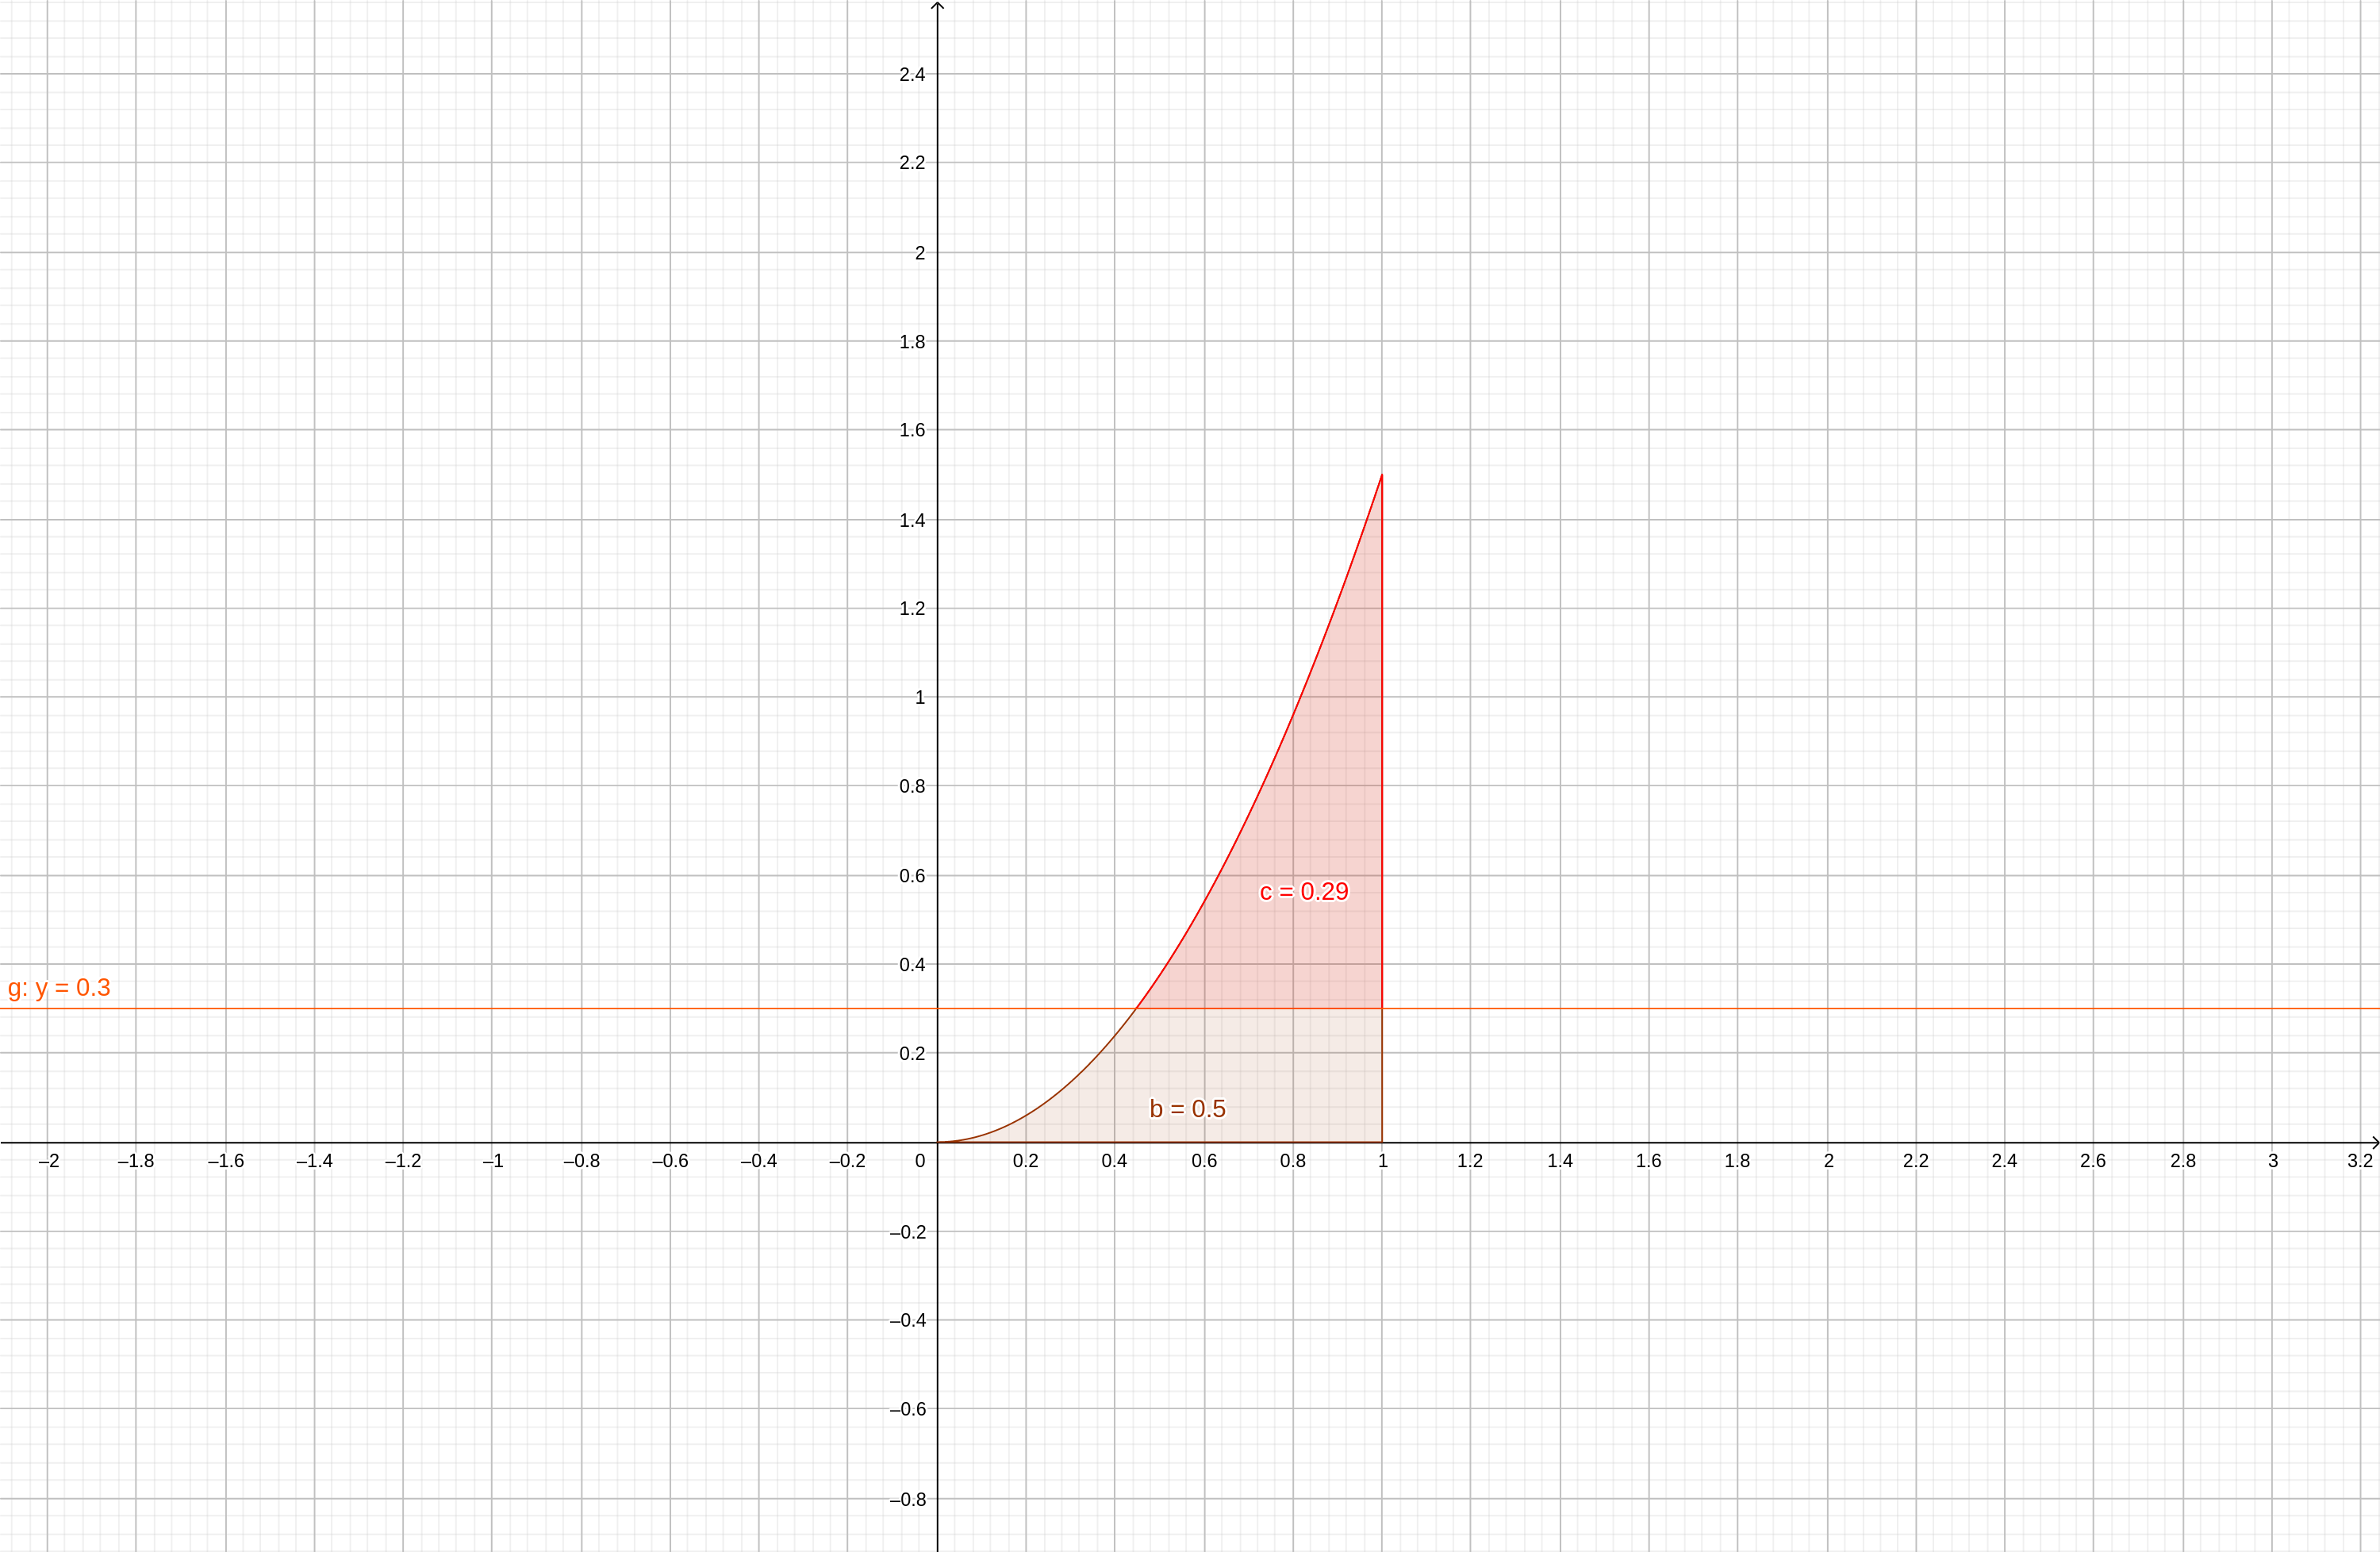
\includegraphics[height=10cm]{TrägermengeUndEreignis.png}\\

\end{document}
